\documentclass[a4paper,10pt]{article}
\usepackage{lmodern}
%\usepackage[czech]{babel}
\usepackage[T1]{fontenc}
\usepackage[utf8]{inputenc}
\usepackage{graphicx}
\usepackage{float}
% \usepackage[top=0.5cm,bottom=2cm,left=1cm,right=1cm]{geometry}
\usepackage{booktabs}
\usepackage{amsmath}
\usepackage{tabularx}
\usepackage{ltablex}
\usepackage{booktabs}
\usepackage{nicematrix}
\usepackage{pdflscape}
\usepackage{hyperref}
\hypersetup{
     colorlinks=true, % Otherwise the links are in color boxes.
     linkcolor=black, % E.g. hyperlinks in table of contents.
     citecolor=black,
     urlcolor=black, % Classical blue web links.
     }

\title{Could Hofstede Guess Your Language?}
\date{\today}
\author{Jaroslav Langer \thanks{langeja5@cvut.cz}}

\begin{document}
\makeatletter
\begin{titlepage}
    \begin{center}
        \vspace*{1cm}
        \Huge{\textbf{\@title}}
        \vspace{0.5cm}

        \LARGE{Predicting a Country's Language Based on Its Cultural Dimensions}
        \vspace{1.5cm}

        \textbf{\@author}
        \@thanks
        \vfill
        Term paper from course\\
        World Economy and Business
        \vspace{0.8cm}

        \Large{Faculty of Information Technology\\
               Czech Technical University in Prague\\
               \@date}
    \end{center}
\end{titlepage}
\makeatother

\begin{abstract}
In this paper I conducted two experiments about inferring country's language from its Hofstede's cultural dimensions.
The first one is more focused analyzing and validating such activity.
In contrast the second experiment tries to accomplish serious predicting abilities.
Most of the model assumptions are slightly violated.
However the second experiment showed it is possible to predict country's language based on its cultural dimensions with reasonable accuracy.

% I am exploring possibility of approximation Hofstede's cultural dimensions using the country's language.
% Because of the dimensions' dataset size I use custom language groups instead of languages itself.
% As a statistical model I chose Gaussian Naive Bayes.
% For evaluation I used Matthews correlation coefficient.

\textbf{Keywords}: Cultural Dimensions; Hofstede; Language; Gaussian Naive Bayes
\end{abstract}

\section{Introduction}
% In 1991 Richard Franke, Geert Hofstede and Michael Bond wrote that "(Cultural indices) explain more than 50 percent of the international differences in economic growth"[Franke 1991].
% How can a culture play such a vital role in a country's development?
% One explanation can come from Mancur Olson, Jr.
% He divides it into marketable i.e. "personal culture" such as skills and public good i.e. "civic culture" that affects one's income only by influencing public policies and institutions[Olson 1996].
% In other words a person's culture  impacts directly his/her life, and also cumulatively and indirectly impacts fellow citizens' lives through institutions.
% Measuring a culture is undeniably an intricate matter.
% Fortunately Geert Hofstede iterated on his research of cultural dimensions until the 3rd edition of Cultures and Organizations[Hofstede 2010].
% In this book we are given 6 time-proven and curated cultural dimensions.
% What is more, for research purposes Geert freely distributes the full dataset [geerthofstede.com].
% The only downside is, the dataset is from 2015 and what is even worse, quite some values are missing.
% This leads to the question: do we need all six dimensions for useful insights?
% More specifically can we use a language as an effective proxy to these dimensions?\cite{hofstede2010cultures}.
Relation between culture and a language is anything but simple.
In the words of Michael Minkov ``Language is a particularly interesting phenomenon.
Traditionally, anthropologists viewed it as part of culture.
Murdock (1940) stated that grammatical rules are cultural because they represent collective habits.
Yet, comparative linguists followed a different tradition,
attempting to explain grammatical differences as if grammar were a closed system,
totally detached from societal features''\cite{minkov2013}
Among the most famous proponents of the traditional view belongs Benjamin Lee Whorf.
This following idea was latter called after him, Whorfism:
``From this fact proceeds what I have called the "linguistic relativity principle,"
which means, in informal terms,
that users of markedly different grammars are pointed by their grammars toward different types of observations and different evaluations of externally similar acts of observation,
and hence are not equivalent as observers but must arrive at somewhat different views of the world''\cite{whorf1956} %page 221
This idea was supported countless times. A recent example may be:
% "IND, at least as measured by Hofstede’s index, is a function of GNP per capita, LAT, and DROP. Affluence, climate, and language use, or both material and symbolic factors, contrib- ute to the country-level IND"
% "If language can be regarded as providing symbolic tools with which a people construct their symbolic world through which their material environment is rendered meaningful, this symbolic world may be able to mod- ify the way in which the material world is understood. Economic affluence and climate may be an inescapable material environment, but its meaning for a people may be significantly shaped by the symbolic tools such as language that they have routinely available."
``Furthermore, the relationship between the material environment and culture seems to depend on the symbolic environment, whatever the causal relationship among these variables. In short, nonmaterial, intangible, symbolic factors do matter in our cultural lives. One of the major symbolic factors that provides an enduring effect on culture may be language, which is, after all, a vast repository that encodes the cumulative wisdom of a people.''\cite{kashima2003}.
The introduction started with Minkov announcing both sides so let him stand on the other end: ``Minkov’s (2006) research concurred with this finding; his historical analysis of English and Scandinavian languages from the early Middle Ages to the present day showed that grammatical change can follow economic and cultural change.''\cite{minkov2013}.
I.e. the change of a language is possible.
Even more radical light on this problem shed Daniel L. Everett with his results of studding old Brazilian culture Pirah\~{a}.
``Pirah\~{a} thus provides striking evidence for the influence of culture on major grammatical structures, contradicting Newmeyer’s (2002:361) assertion (citing “virtually all linguists today”), that “there is no hope of correlating a language’s gross grammatical properties with sociocultural facts about its speakers.” If I am correct, Pirah\~{a} shows that gross grammatical properties are not only correlated with sociocultural facts but may be determined by them.``
I will not try to figure out any underlying relationship of culture and language.
Instead, I will test following:

\noindent\textbf{Hypothesis}: Cultural dimensions contain sufficient information to identify a country's language.

\noindent\textbf{Verification criteria}: Gaussian Naive Bayes can correctly classify language for most of the countries.

\section{Theoretical Part}

The question of whether the culturally similar countries share the same language was usually approached with some kind of clustering.
Originally, Hofstede clustered the countries into 12 groups and stated ``the culture patterns found go across language families''\cite{hofstede2001}. %pp. 49, 62-65
Clustering method is very dependent on parameters such as number of clusters, distance metric, from what point to measure the metric for a cluster e.g. from center, from border etc.
So unsurprisingly other clustering results arose as well.
One of the more influential was from Simcha Ronen who wrote ``Language is another dimension underlying the clusters. A language contains meanings and values that are likely to influence individuals' work goals. For the most part, the countries in each cluster share a language or language group.``\cite{ronen1985}.
To avoid misunderstanding, in both works the language or language family was shared by the cluster. Hofstede moreover argued it is not the only cause as there are also groups across language families.
Another paper from Linghui Tang says ``Language is an important element to define cultural clusters. In particular, countries that use pronoun drop languages (Arabic, Spanish, and most Asian languages) have lower individualism and higher power distance scores. The languages with more than two second-person singular pronouns (Arabic, German, and Spanish) have higher uncertainty avoidance scores.''\cite{tang2008}.
It refers to the publications from Kashima \cite{kashima1998, kashima2003} disputed by Minkov\cite{minkov2013} as I already mentioned.
However the most similar problem was approached by Minkov with Hofstede when tackling the question whether "Is National Culture a Meaningful Concept?"
There they clustered regions and concluded that as most of the clusters somehow overlaps with national borders it is a meaningful to talk about culture in terms of nations. Interesting quote for this purpose is ``The role of the English language as a cultural unifier is also worth exploring, although our results for Latin America and China/Taiwan suggest that a shared language is not enough to create close cultural similarities.''\cite{minkov2011}.

Having said all this, clustering is a great technique that can bring a lot of insight.
On the other hand its sensitivity to parameters makes it more suitable for experts with long experience.
I chose to try a different approach. As Hofstede mentioned ``A model in which worldwide differences in national cultures are categorized according to five independent dimensions''\cite{hofstede1993}. I am going to take it literally and assume the cultural dimensions to be (more-or-less) independent.
Then I am going to further assume the dimensions are normally distributed.
Assuming these properties I can use the Gaussian Naive Bayes Classifier.

\subsection{Gaussian Naive Bayes Classifier}

\begin{figure}[H]
    \begin{align}
    p(k \mid \mathbf{x}) &= {\frac {p(k)\ p(\mathbf{x} \mid k)}{\sum_{k\in K}p(k)\ p(\mathbf{x} \mid k)}} \\
    p(x=x_i \mid k) &={\frac {1}{\sqrt {2\pi \sigma_{k,i}^{2}}}} e^{- \frac{(x_i - \mu_{k,i})^2}{2\sigma _{k,i}^2}} \\
    p(\mathbf{x} \mid k) &= \prod_{x_i \in \mathbf{x}}\ p(x_{i} \mid k) \\
    k &= \underset{\{k\in K\}}{\operatorname{argmax}}\left(\ p(k) \prod_{x_i \in \mathbf{x}}\ p(x_{i} \mid k)\right)
    \end{align}
    \caption{Gaussian Naive Bayes key equations}
    \label{bayes}
\end{figure}

In short, Gaussian Naive Bayes uses Bayes Theorem and Law of total probability to calculate probability of class $k$ given random vector $\mathbf{x}$ (of cultural dimensions) equation (1).
For every class $k$ it assumes every dimension $i$ of vector $x$ to be independent and normally distributed.
When this is satisfied it can learn parameters of normal distribution $\mu_{k,i},\ \sigma_{k,i}$, for every dimension $i$ and class $k$.
The probability of $x_i$ (cultural dimension) for class $k$ is then given by equation (2).
As the dimensions are independent the probability of random vector $\mathbf{x}$ (cultural dimensions) for class $k$ is given by the equation (3).
The equation (4) classifies every random (cultural) vector $\mathbf{x}$ into class $k$.
It emerges when we substitute equation (3) into the dividend of equation (1).
And instead of calculating equation (1) only for one class $k$, we calculate it for all the classes and take the biggest value (argmax).
Last modification is that we leave out the divisor.
It would be the same value for all the classes $k$ so we can omit it and it doesn't affect the maximum.
Better explanation can be found here\cite{cornellBayes}.

\subsection{Confusion Matrix and Accuracy}

After the classifier is trained, I am going to construct a confusion matrix.
It is a matrix with True values in columns and Predicted values in rows.
It may look perhaps like this:

\begin{center}
\begin{tabular}{ c|c c }
            & Reality \\
    Prediction & First & Second \\
    \hline
    First      & 1     & 2\\
    Second     & 3     & 4\\
\end{tabular}
\end{center}

In this example the first class was correctly predicted ones.
The second class was correctly classified 4 times.
It happened twice, that the second class was classified as the first one.
With three cases the first class was classified as the second one.

The \textbf{accuracy} is calculated as number of correctly classified divided by the total amount.
So in this example it would be $\frac{1+4}{(1+4)+(2+3)} = \frac{5}{5+5} = \frac{1}{2} = 0.5$

\section{Practical Part}

I downloaded Hofstede's cultural dimension data\cite{hofstedeData}.
The dataset contains 111 entries.
78 data points don't miss a single value neither of these dimensions: PDI, IDV, MAS and UAI.
Apparently these data come from the original survey.
The Long-Term Orientation and Indulgence came later, so they both miss some values independently.
As I want to do a prediction of a language I am going to use all the data including the language differentiated.
E.g. Canada, Canada French, or Belgium French, Belgium Netherlands etc.
If such data point misses only one or two dimension values I am going to fill it from the closest point/s.
Later I am going to assume the the dimensions to be independent, let's for a start see its' correlations.

\begin{figure}[H]
       \begin{center}
              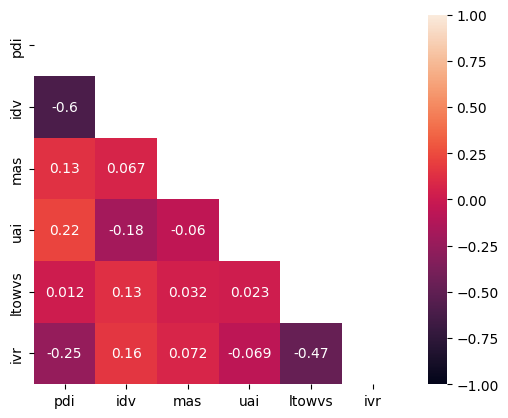
\includegraphics[width=6cm]{../figures/dimension_correlations.png}
       \end{center}
       \caption{Dimension Correlations}
\end{figure}

Evidently the couples IDV-PDI and LTO-IVR are strongly negatively correlated.
It is the end of my dream about independent dimensions.
However let's continue anyway.

In order to obtain knowledge about which languages are spoken in a country I turned to the CIA factbook\cite{ciaFactbook}.
Most of the languages are spoken only in few (one or two) countries.
I am going to overcome it by first "clustering" the languages based on their relatedness.
Such information is available at Ethnologue\cite{ethnologue}.

I started with following clusters.
They are nowhere near an ideal ones.
I just want to have a sensible sized groups (e.g. 10 observations) to see if any reasonable results can be obtained.

\begin{figure}[H]
\begin{longtable}[]{@{}lr@{}}
\toprule
Language Group & Count \\
\midrule
\endhead
Spanish & 15 \\
Germanic & 15 \\
Balto-Slavic & 15 \\
African & 12 \\
Romance & 10 \\
English & 10 \\
Semitic & 9 \\
----------------- & \\
Indo-Iranian & 4 \\
Palaeo-Balkan & 3 \\
Turkic & 3 \\
Sino-Tibetan & 3 \\
Uralic & 3 \\
Malayo-Polynesian & 3 \\
\bottomrule
\end{longtable}
\caption{Language groups of adequate sample size.}
\end{figure}

For details about the countries used and their languages see appendix Figure \ref{langs1}.

Having these clusters let's look at the cultural dimension distributions.

\begin{figure}[H]
       \begin{center}
              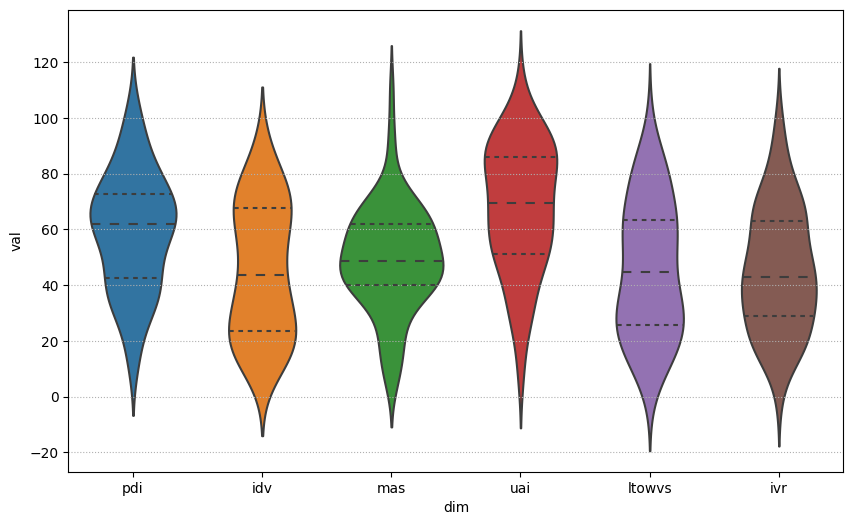
\includegraphics[width=10cm]{../figures/dim_distributions.png}
       \end{center}
       \caption{Dimension Distributions}
\end{figure}

Fortunately it looks somehow normal, let's look at outliers.

\subsection{Outliers Detection}

\begin{figure}[H]
       \begin{center}
              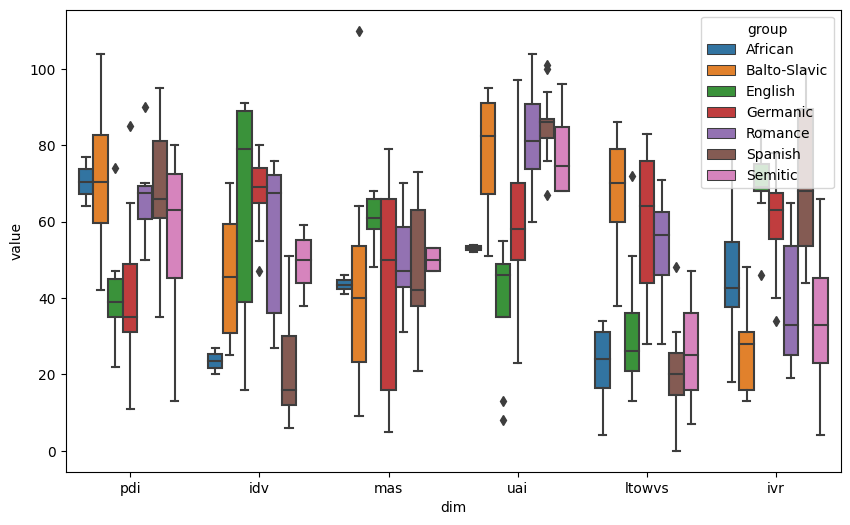
\includegraphics[width=12cm]{../figures/dim_overview.png}
       \end{center}
       \caption{Outliers Overview}
       \label{overview}
\end{figure}

Traditional assessment of outliers based on a multiple of interquartile range would mark some of these data points as outliers.
However given the fact that the data points are valid in the other dimensions i.e. they are vectors, so the only one component is laying out.
And considering the limitations of available amount of data.
I chose to not remove any data point.
Following figures visualizes the dimensions with pinpointing several countries.
They are not all outliers, if you are interested in which of them are (by the conventional view) compare the points with the previous figure \ref{overview}.
The figures are quite small, but the information is there.
These figures are more about getting in touch with the data.

\begin{figure}[H]
       \begin{center}
              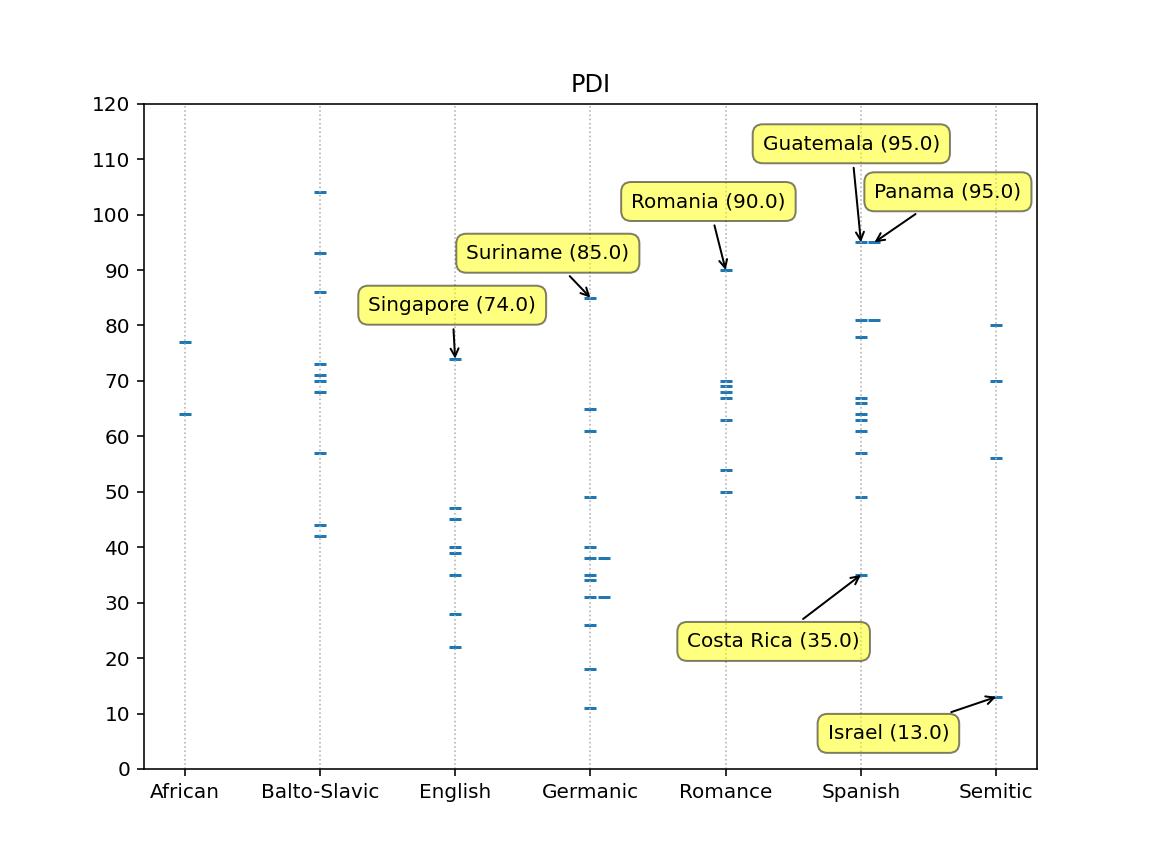
\includegraphics[width=6cm]{../figures/pdi.png}
              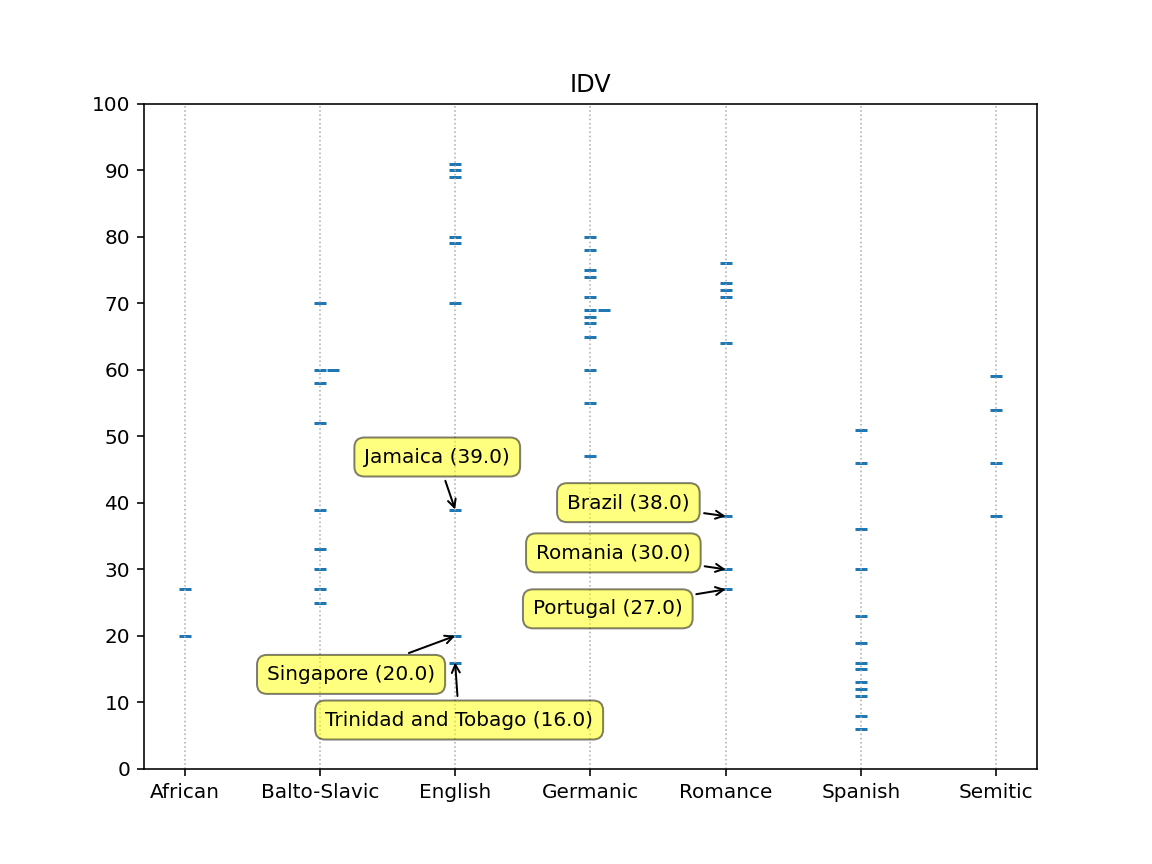
\includegraphics[width=6cm]{../figures/idv.png}
              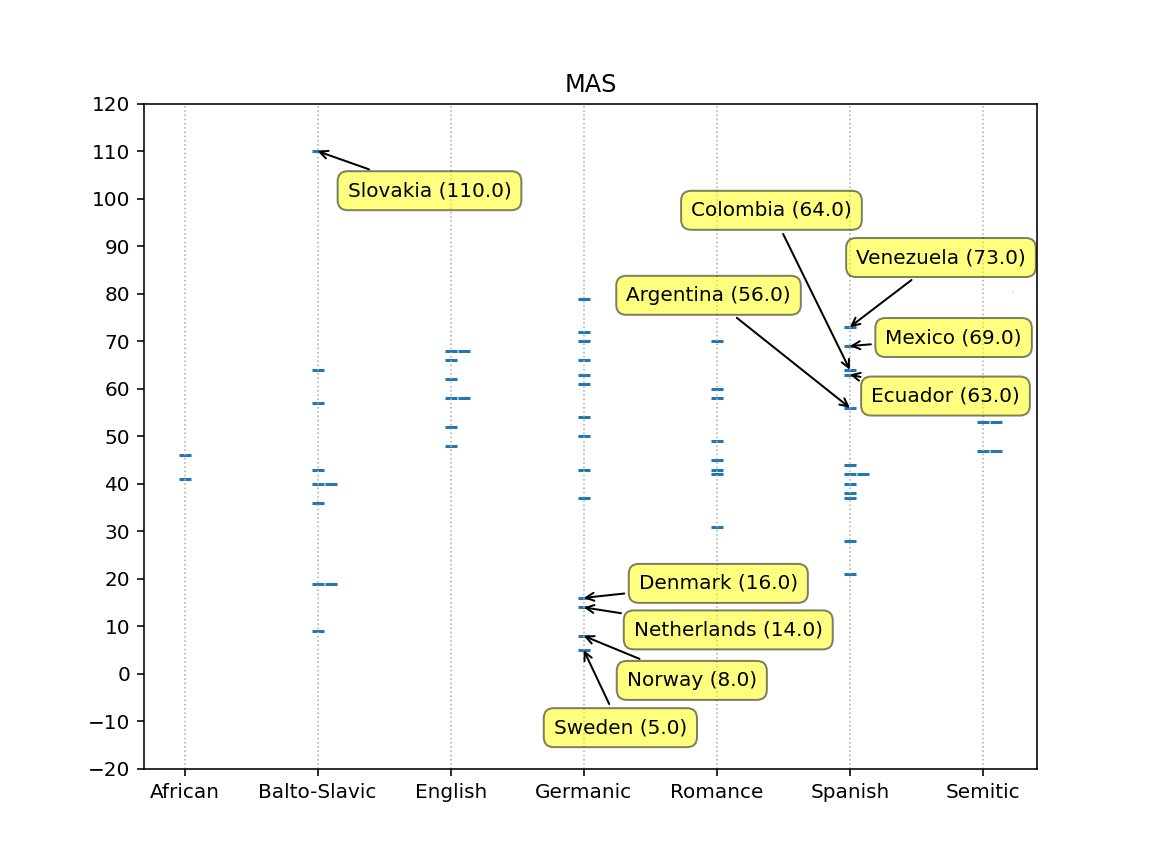
\includegraphics[width=6cm]{../figures/mas.png}
              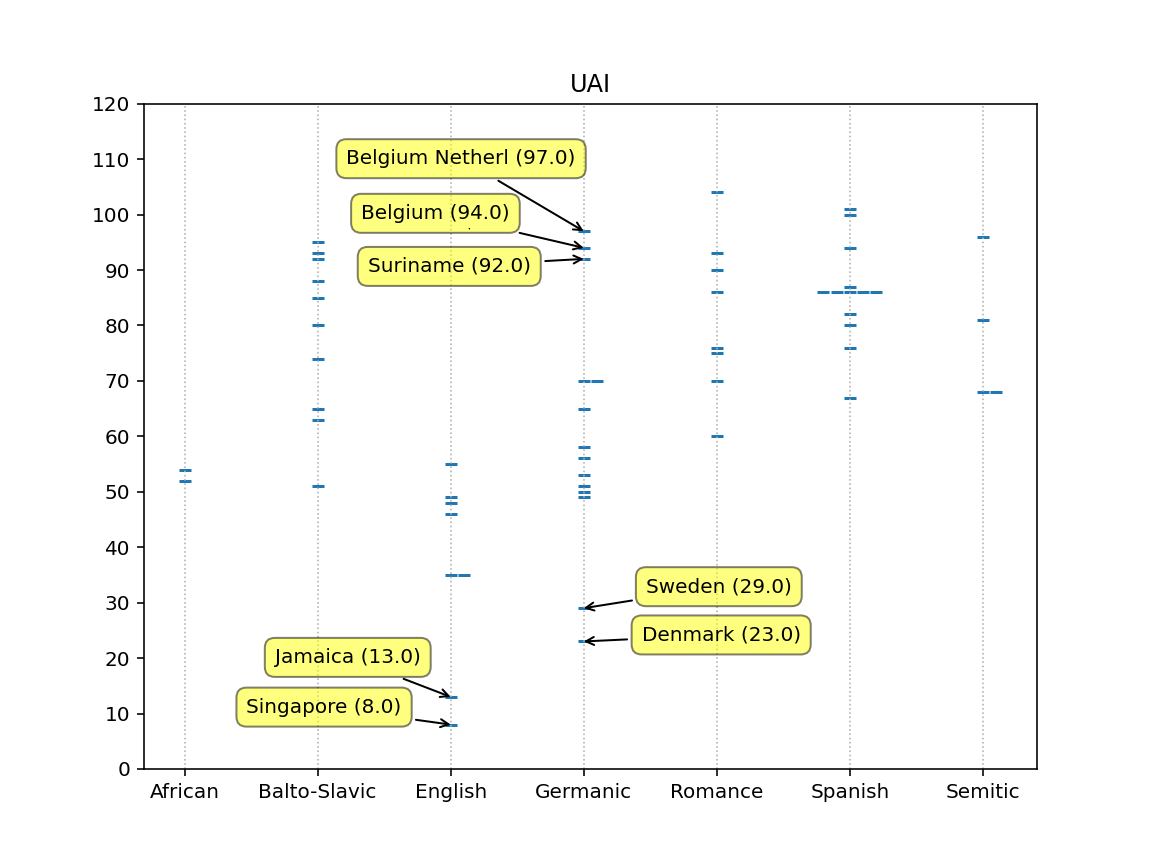
\includegraphics[width=6cm]{../figures/uai.png}
              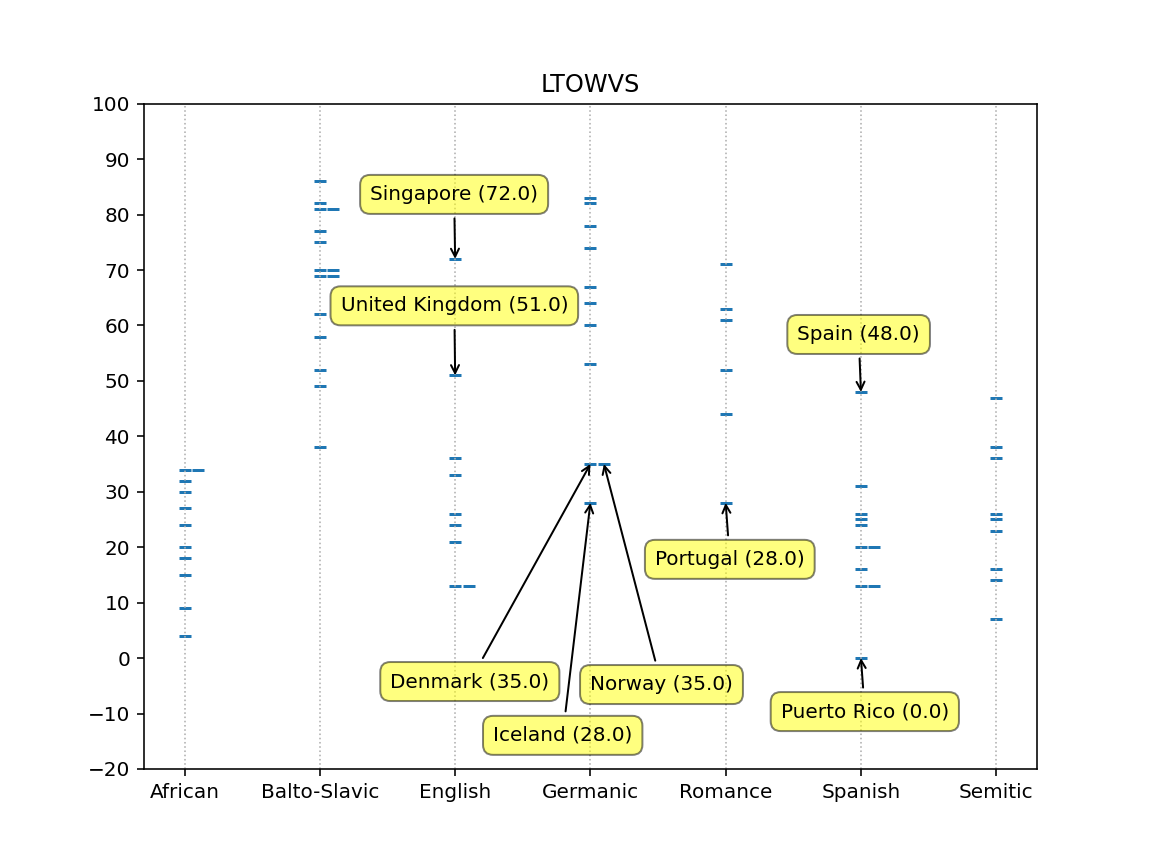
\includegraphics[width=6cm]{../figures/lto.png}
              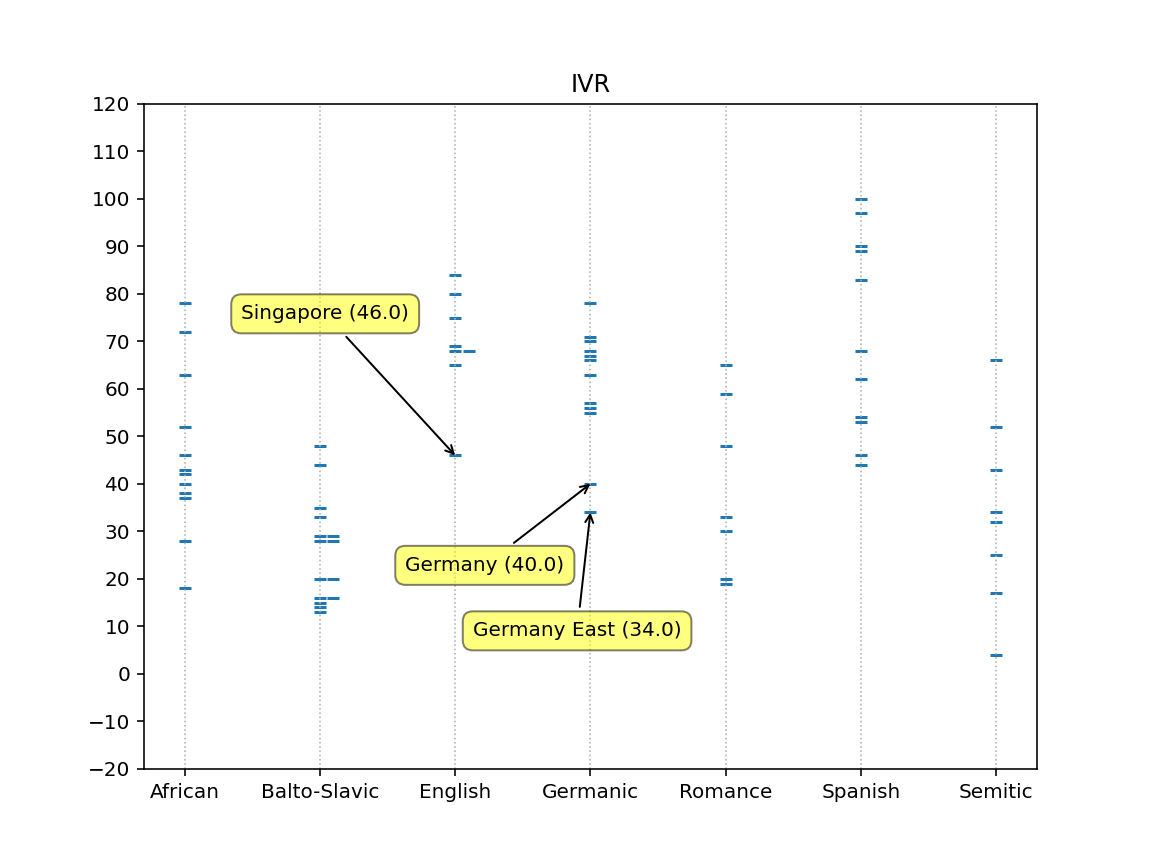
\includegraphics[width=6cm]{../figures/ivr.png}
       \end{center}
       \caption{Data points which stand out. Not all highlighted data points are outliers. Some points are shown just for a context.}
\end{figure}

Now let's statistically test whether the data are drawn from normal distributions.
For this purpose I will use both Anderson–Darling and Kolmogorov–Smirnov normality tests.

\begin{longtable}[]{@{}lll@{}}
\toprule
dim & ks test & ad test \\
\midrule
\endhead
pdi & 0.548837 & 0.503694 \\
idv & 0.0357113 & 0.000591842 \\
mas & 0.268814 & 0.15928 \\
uai & 0.0384659 & 0.0495701 \\
ltowvs & 0.0215968 & 0.00959888 \\
ivr & 0.495077 & 0.13018 \\
\bottomrule
\end{longtable}

Individuality, Uncertainty Avoidance and Long-term Orientation have all very low p-value.
So it is possible to reject their normality.
However I want to assume it for further steps, so let's just keep it in mind and keep going.

Assuming the dimensions' distributions to be normal it makes sense to test if the language dimensions have significantly different expected values (means).
I don't need all pairs to have significantly different means in all dimensions.
It should be sufficient for each pair of languages to have a significantly different expected value in at least one dimension.
In order to examine this I will use Welch's t-test.
Success would be if I reject the null hypothesis for each pair of languages in some dimension.

\subsection{Pair-wise T-test}

\begin{figure}[H]
       \begin{center}
              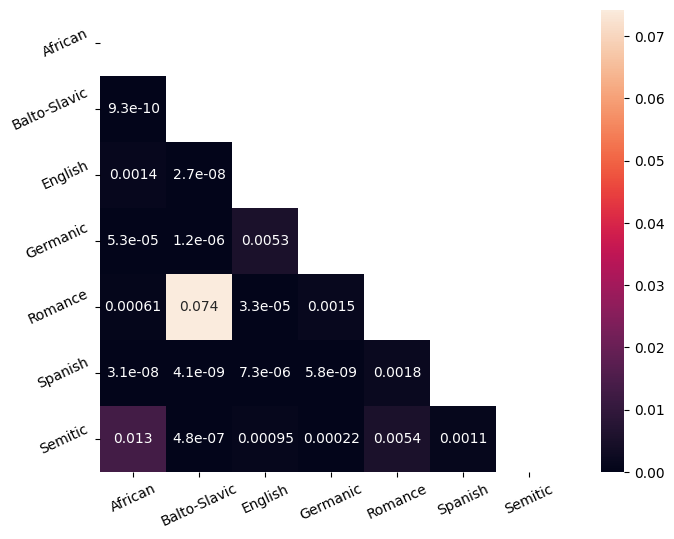
\includegraphics[width=6cm]{../figures/test_mean_difference.png}
       \end{center}
       \caption{Test of different mean values. For every pair, there is visualized the lowest p-value across all dimensions.}
\end{figure}

There is no dimensions in which the Balto-Slavic and Romance groups have significantly (5\%) different expected value.
Let's keep it in mind, and ignore it.

So, when assuming to have independent normally distributed and separable exogenous variables, it should be possible to fit the Gaussian Naive Bayes model with perfect scores. Let's train it and see the confusion matrix.

\subsection{Confusion Matrix}

\begin{figure}[H]
\begin{longtable}[]{@{}lrrrrrrr@{}}
\toprule
    & African & Balto-Slavic & English & Germanic & Romance & Semitic & Spanish \\
\midrule
\endhead
African & 12 & 0 & 0 & 0 & 0 & 0 & 0 \\
Balto-Slavic & 0 & 13 & 0 & 0 & 2 & 0 & 0 \\
English & 0 & 0 & 10 & 0 & 0 & 0 & 0 \\
Germanic & 0 & 0 & 0 & 13 & 0 & 0 & 0 \\
Romance & 0 & 2 & 0 & 2 & 7 & 1 & 1 \\
Semitic & 0 & 0 & 0 & 0 & 0 & 8 & 0 \\
Spanish & 0 & 0 & 0 & 0 & 1 & 0 & 14 \\
\bottomrule
\end{longtable}
\caption{Confusion matrix of the first experiment. For details about the confusions and its probabilities see appendix.}
\end{figure}

This confusion matrix equals to \textbf{accuracy} of $0.895$.
This looks promising.
A biggest disadvantage of this model is probably the fact it actually does not predict languages.
Instead it predicts clusters that are honestly quite big.
What is even worse there are a lot of countries omitted from the sample, which simplifies the task significantly.

Let's now take different path and instead of groups of 10 samples, let's divide the countries such that there will be high number of languages or small groups of about 3 observations.


\begin{figure}[H]
\begin{longtable}[]{@{}lr@{}}
\toprule
Language Group & Count \\
\midrule
\endhead
West-Iberian       & 15 \\
English            & 10 \\
Ungrouped          &  7 \\
Romance            &  6 \\
Semitic            &  4 \\
German             &  4 \\
Indo-Iranian       &  4 \\
Slavic/South       &  4 \\
Dutch              &  3 \\
Chinese            &  3 \\
Slavic/West        &  3 \\
Germanic/North     &  3 \\
Uralic             &  3 \\
Malayo-Polynesian  &  3 \\
Balto-Slavic/East  &  3 \\
\bottomrule
\end{longtable}
\caption{Groups of three or more samples for the closest languages possible. See Figure \ref{langs2} for complete language listing.}
\end{figure}

It does not contain all the languages as some of them were removed because of missing values.
When you have 10 samples, it is fine, if some of it is missing value in some dimension.
For sample size of three it is intolerable.
Statistical properties of such experiment are becoming a question.
However if this works, the properties can be studied later, if not, it is irrelevant.


When the Gaussian Naive Bayes was trained on these samples, the accuracy on the same data was $0.827$.
Which is somewhat surprising considering the number of possible languages to predict.
What is better, the prediction errors mostly "make sense" such as predicting Estonia to be Balto-Slavic/East (together with its neighbors) while the correct group was Uralic. Or predicting Singapore as Chinese also feels excusable. For details see Figure \ref{confmat2} in appendix. 

\section{Conclusion}

It is possible to predict most ($0.827$) of the small language groups correctly using the Gaussian Naive Bayes classifier based on cultural dimensions.
However talking about predicting when the learning was done on the same data as the evaluation is optimistic to say the least.
Also I didn't try to control any variables such as geography.
Additionally there are no clues about performance of such prediction of other variable.
In this regard, this work seems novel in a way it is not doing cluster analysis and instead it builds probabilistic model for predictions.
Such model is of course of no use, as we already know the correct languages, nevertheless there could be locked potential to predict something else.
For now, I showed the Hofstede's dimensions contain enough information about the language it is possible to "guess" it with a high accuracy.

\bibliographystyle{apalike}
\bibliography{refs}

\appendix

\section{First Experiment}

\subsection{Languages}

\begin{figure}
\begin{longtable}[]{@{}lll@{}}
\toprule
Country & Language & Group \\
\midrule
\endhead
Africa East & Niger--Congo & African \\
Uganda & English, Arabic & African \\
Tanzania & Kiswahili or Swahili & African \\
South Africa & African & African \\
Rwanda & Kinyarwanda & African \\
Mali & French, Bambara & African \\
Zambia & African & African \\
Ghana & Asante, Ewe, Fante, Boron & African \\
Ethiopia & Oromo, Amharic & African \\
Burkina Faso & African & African \\
Zimbabwe & African & African \\
Africa West & Niger--Congo & African \\
Latvia & Latvian, Russian & Balto-Slavic \\
North Macedonia & Macedonian, Albanian & Balto-Slavic \\
Montenegro & Serbian, Montenegrin & Balto-Slavic \\
Poland & Polish & Balto-Slavic \\
Russia & Russian & Balto-Slavic \\
Serbia & Serbian & Balto-Slavic \\
Slovakia & Slovak & Balto-Slavic \\
Slovenia & Slovene & Balto-Slavic \\
Czechia & Czech & Balto-Slavic \\
Belarus & Slavic & Balto-Slavic \\
Bulgaria & Bulgarian & Balto-Slavic \\
Bosnia and Herzegovina & Balto-Slavic & Balto-Slavic \\
Ukraine & Ukrainian, Russian & Balto-Slavic \\
Croatia & Croatian & Balto-Slavic \\
Lithuania & Lithuanian & Balto-Slavic \\
Australia & English & English \\
Jamaica & English & English \\
Ireland & English & English \\
New Zealand & English & English \\
United Kingdom & English & English \\
Nigeria & English & English \\
Canada & English & English \\
United States & English & English \\
Singapore & English & English \\
Trinidad and Tobago & English & English \\
Norway & Norwegian & Germanic \\
Switzerland German & German & Germanic \\
Netherlands & Dutch & Germanic \\
Suriname & Dutch & Germanic \\
Sweden & Swedish & Germanic \\
South Africa white & Germanic & Germanic \\
Switzerland & German, French & Germanic \\
Belgium Netherl & Germanic & Germanic \\
Germany & German & Germanic \\
Austria & Germanic & Germanic \\
Denmark & Danish & Germanic \\
Germany East & Germanic & Germanic \\
Iceland & Icelandic & Germanic \\
Belgium & Germanic & Germanic \\
Luxembourg & Luxembourgish & Germanic \\
Italy & Italian & Romance \\
Canada French & French & Romance \\
Switzerland French & French & Romance \\
Belgium French & Romance & Romance \\
Andorra & Catalan & Romance \\
Brazil & Portuguese & Romance \\
Portugal & Portuguese & Romance \\
France & French & Romance \\
Romania & Romanian & Romance \\
Moldova & Romanian & Romance \\
Algeria & Arabic & Semitic \\
Egypt & Arabic & Semitic \\
Jordan & Arabic & Semitic \\
Arab countries & Arabic & Semitic \\
Malta & Maltese & Semitic \\
Morocco & Arabic & Semitic \\
Israel & Hebrew & Semitic \\
Saudi Arabia & Arabic & Semitic \\
Iraq & Arabic, Kurdish & Semitic \\
Spain & Spanish & Spanish \\
Dominican Republic & Spanish & Spanish \\
Guatemala & Spanish & Spanish \\
Costa Rica & Spanish & Spanish \\
Panama & Spanish & Spanish \\
Colombia & Spanish & Spanish \\
Peru & Spanish & Spanish \\
Chile & Spanish & Spanish \\
El Salvador & Spanish & Spanish \\
Puerto Rico & Spanish & Spanish \\
Argentina & Spanish & Spanish \\
Uruguay & Spanish & Spanish \\
Venezuela & Spanish & Spanish \\
Ecuador & Spanish & Spanish \\
Mexico & Spanish & Spanish \\
\bottomrule
\end{longtable}
\label{langs1}
\end{figure}

\subsection{Probabilities of Misclassified Countries}

\begin{landscape}
\begin{tabularx}{\textwidth}{llllllllll}
\toprule
    Country & Group & Prediction & African & Balto-Slavic & English & Germanic & Romance & Semitic & Spanish \\
\midrule
\endhead
Bosnia and Herzegovina & Balto-Slavic & Romance & 0 & 0.48 & 2.17e-07 & 0.002 & 0.52 & 0.0001 & 8.05e-07 \\
Poland & Balto-Slavic & Romance & 0 & 0.11 & 1.28e-07 & 0.002 & 0.89 & 2.64e-11 & 0.0009 \\
Belgium Netherl & Germanic & Romance & 0 & 0.0005 & 4.03e-06 & 0.34 & 0.66 & 4.66e-11 & 2.48e-07 \\
Suriname & Germanic & Romance & 0 & 0.07 & 2.56e-08 & 0.017 & 0.91 & 9.82e-11 & 0.002 \\
Moldova & Romance & Balto-Slavic & 0 & 0.78 & 5.88e-11 & 4.73e-05 & 0.22 & 0.004 & 2.51e-09 \\
Portugal & Romance & Spanish & 0 & 0.04 & 1.29e-11 & 1.93e-07 & 0.13 & 3.54e-23 & 0.83 \\
Romania & Romance & Balto-Slavic & 0 & 0.89 & 1.92e-13 & 2.48e-09 & 0.11 & 2.70e-07 & 0.0007 \\
Malta & Semitic & Romance & 0 & 0.0003 & 0.0002 & 0.38 & 0.59 & 0.03 & 0.004 \\
Spain & Spanish & Romance & 0 & 0.06 & 1.08e-06 & 0.01 & 0.92 & 0.0008 & 0.001 \\
\bottomrule
\end{tabularx}
\end{landscape}

\section{Second Experiment}

\subsection{Languages}

\begin{figure}
\begin{center}
\begin{tabularx}{\textwidth}{llX}
\toprule
country &              group &                                          languages \\
\midrule
Africa East         &          Ungrouped &                                                NaN \\
Africa West         &            English &                                                NaN \\
Arab countries      &            Semitic &                                                NaN \\
Argentina           &       West-Iberian &  Spanish (official), Italian, English, German, ... \\
Australia           &            English &  English 72.7\%, Mandarin 2.5\%, Arabic 1.4\%, Can... \\
Austria             &             German &  German (official nationwide) 88.6\%, Turkish 2.... \\
Bangladesh          &       Indo-Iranian &  Bangla 98.8\% (official, also known as Bengali)... \\
Belgium French      &            Romance &                                                NaN \\
Belgium Netherl     &              Dutch &                                                NaN \\
Brazil              &       West-Iberian &  Portuguese (official and most widely spoken la... \\
Bulgaria            &       Slavic/South &  Bulgarian (official) 76.8\%, Turkish 8.2\%, Roma... \\
Canada              &            English &  English (official) 58.7\%, French (official) 22... \\
Canada French       &            Romance &                                                NaN \\
Chile               &       West-Iberian &  Spanish 99.5\% (official), English 10.2\%, Indig... \\
China               &            Chinese &  Standard Chinese or Mandarin (official; Putong... \\
Colombia            &       West-Iberian &                                 Spanish (official) \\
Costa Rica          &       West-Iberian &                        Spanish (official), English \\
Croatia             &       Slavic/South &  Croatian (official) 95.6\%, Serbian 1.2\%, other... \\
Czechia             &        Slavic/West &  Czech (official) 95.4\%, Slovak 1.6\%, other 3\% ... \\
Denmark             &     Germanic/North &  Danish, Faroese, Greenlandic (an Inuit dialect... \\
Ecuador             &       West-Iberian &  Spanish (Castilian) 93\% (official), Quechua 4.... \\
El Salvador         &       West-Iberian &  Spanish (official), Nawat (among some Amerindi... \\
Estonia             &             Uralic &  Estonian (official) 68.5\%, Russian 29.6\%, Ukra... \\
Finland             &             Uralic &  Finnish (official) 86.9\%, Swedish (official) 5... \\
France              &            Romance &  French (official) 100\%, declining regional dia... \\
Germany             &             German &  German (official); note - Danish, Frisian, Sor... \\
United Kingdom      &            English &                                            English \\
Greece              &          Ungrouped &  Greek (official) 99\%, other (includes English ... \\
Guatemala           &       West-Iberian &  Spanish (official) 69.9\%, Maya languages 29.7\%... \\
Hong Kong           &            Chinese &  Cantonese (official) 88.9\%, English (official)... \\
Hungary             &             Uralic &  Hungarian (official) 99.6\%, English 16\%, Germa... \\
India               &       Indo-Iranian &  Hindi 43.6\%, Bengali 8\%, Marathi 6.9\%, Telugu ... \\
Indonesia           &  Malayo-Polynesian &  Bahasa Indonesia (official, modified form of M... \\
Iran                &       Indo-Iranian &  Persian Farsi (official), Azeri and other Turk... \\
Ireland             &            English &  English (official, the language generally used... \\
Israel              &            Semitic &  Hebrew (official), Arabic (special status unde... \\
Italy               &            Romance &  Italian (official), German (parts of Trentino-... \\
Jamaica             &            English &                            English, English patois \\
Japan               &          Ungrouped &                                           Japanese \\
Korea, South        &          Ungrouped &  Korean, English (widely taught in elementary, ... \\
Latvia              &  Balto-Slavic/East &  Latvian (official) 56.3\%, Russian 33.8\%, other... \\
Lithuania           &  Balto-Slavic/East &  Lithuanian (official) 82\%, Russian 8\%, Polish ... \\
Luxembourg          &             German &  Luxembourgish (official administrative and jud... \\
Malaysia            &  Malayo-Polynesian &  Bahasa Malaysia (official), English, Chinese (... \\
Malta               &            Semitic &  Maltese (official) 90.1\%, English (official) 6... \\
Mexico              &       West-Iberian &  Spanish only 93.8\%, Spanish and indigenous lan... \\
Morocco             &            Semitic &  Arabic (official), Berber languages (Tamazight... \\
Netherlands         &              Dutch &  Dutch (official); note - Frisian is an officia... \\
New Zealand         &            English &  English (de facto official) 95.4\%, Maori (de j... \\
Norway              &     Germanic/North &  Bokmal Norwegian (official), Nynorsk Norwegian... \\
Pakistan            &       Indo-Iranian &  Punjabi 48\%, Sindhi 12\%, Saraiki (a Punjabi va... \\
Panama              &       West-Iberian &  Spanish (official), indigenous languages (incl... \\
Peru                &       West-Iberian &  Spanish (official) 82.9\%, Quechua (official) 1... \\
Philippines         &  Malayo-Polynesian &  unspecified Filipino (official; based on Tagal... \\
Poland              &        Slavic/West &  Polish (official) 98.2\%, Silesian 1.4\%, other ... \\
Portugal            &       West-Iberian &  Portuguese (official), Mirandese (official, bu... \\
Romania             &            Romance &  Romanian (official) 85.4\%, Hungarian 6.3\%, Rom... \\
Russia              &  Balto-Slavic/East &  Russian (official) 85.7\%, Tatar 3.2\%, Chechen ... \\
Serbia              &       Slavic/South &  Serbian (official) 88.1\%, Hungarian 3.4\%, Bosn... \\
Singapore           &            English &  English (official) 48.3\%, Mandarin (official) ... \\
Slovakia            &        Slavic/West &  Slovak (official) 78.6\%, Hungarian 9.4\%, Roma ... \\
Slovenia            &       Slavic/South &  Slovene (official) 87.7\%, Croatian 2.8\%, Serbo... \\
Spain               &       West-Iberian &  Castilian Spanish (official nationwide) 74\%, C... \\
Suriname            &              Dutch &  Dutch (official), English (widely spoken), Sra... \\
Sweden              &     Germanic/North &                                 Swedish (official) \\
Switzerland French  &            Romance &                                                NaN \\
Switzerland German  &             German &                                                NaN \\
Taiwan              &            Chinese &  Mandarin (official), Taiwanese (Min Nan), Hakk... \\
Thailand            &          Ungrouped &  Thai (official) only 90.7\%, Thai and other lan... \\
Trinidad and Tobago &            English &  English (official), Trinidadian Creole English... \\
Turkey              &          Ungrouped &  Turkish (official), Kurdish, other minority la... \\
United States       &            English &  English only 78.2\%, Spanish 13.4\%, Chinese 1.1... \\
Uruguay             &       West-Iberian &                                 Spanish (official) \\
Venezuela           &       West-Iberian &   Spanish (official), numerous indigenous dialects \\
Vietnam             &          Ungrouped &  Vietnamese (official), English (increasingly f... \\
\bottomrule
\end{tabularx}
\end{center}
\label{langs2}
\end{figure}

\subsection{Confusion Matrix}

\begin{landscape}
\begin{figure}[H]
\begin{tabularx}{\textwidth}{XrccccXcXccXXccX}
\toprule
{} &  Bal.-Slav.East &  Chinese &  Dutch &  English &  German &  Ger. North &  Indo-Iran. &  Mal.-Poly &  Romance &  Semitic &  Slav. Sth &  Slav. Wst &  Ungrouped &  Uralic &  West-Iberian \\
\midrule
Balto-Slavic/East &         \textbf{3} &          &        &          &         &                 &               &                    &          &          &               &              &            &       1 &               \\
\midrule
    Chinese           &                    & \textbf{2} &        &        1 &         &                 &               &                    &          &          &               &              &          1 &         &               \\
\midrule
    Dutch             &                    &          & \textbf{2} &          &         &                 &               &                    &          &          &               &              &            &         &               \\
\midrule
    English           &                    &          &        & \textbf{9} &         &                 &               &                    &        1 &          &               &              &            &         &               \\
\midrule
    German            &                    &          &        &          & \textbf{4} &                 &               &                    &          &          &               &              &            &         &               \\
\midrule
    Germanic/North    &                    &          &        &          &         &   \textbf{3}    &               &                    &          &          &               &              &            &         &               \\
\midrule
    Indo-Iranian      &                    &          &        &          &         &                 &  \textbf{3}   &                    &          &        1 &               &              &            &         &               \\
\midrule
    Malayo-Polynesian &                    &          &        &          &         &                 &               &    \textbf{3}      &          &          &               &              &            &         &               \\
\midrule
    Romance           &                    &          &        &          &         &                 &               &                    & \textbf{4} &        1 &               &              &            &         &             1 \\
\midrule
    Semitic           &                    &          &        &          &         &                 &               &                    &          & \textbf{2} &               &              &            &         &               \\
\midrule
    Slavic/South      &                    &          &        &          &         &                 &               &                    &        1 &          & \textbf{4}    &              &            &         &               \\
\midrule
    Slavic/West       &                    &          &        &          &         &                 &               &                    &          &          &               & \textbf{3}   &            &         &               \\
\midrule
    Ungrouped         &                    &        1 &        &          &         &                 &             1 &                    &          &          &               &              & \textbf{5} &         &             1 \\
\midrule
    Uralic            &                    &          &        &          &         &                 &               &                    &          &          &               &              &            & \textbf{2} &               \\
\midrule
    West-Iberian      &                    &          &      1 &          &         &                 &               &                    &          &          &               &              &          1 &         &  \textbf{13}  \\
\bottomrule
\end{tabularx}
\caption{True groups are written as columns, predicted groups are in rows.}
\label{confmat2}
\end{figure}
\end{landscape}

\begin{tabular}{lll}
\toprule
country &         group &         prediction \\
\midrule
Arab countries &       Semitic &       Indo-Iranian \\
Canada French  &       Romance &            English \\
Estonia        &        Uralic &  Balto-Slavic/East \\
Iran           &  Indo-Iranian &          Ungrouped \\
Malta          &       Semitic &            Romance \\
Portugal       &  West-Iberian &          Ungrouped \\
Romania        &       Romance &       Slavic/South \\
Singapore      &       English &            Chinese \\
Spain          &  West-Iberian &            Romance \\
Suriname       &         Dutch &       West-Iberian \\
Taiwan         &       Chinese &          Ungrouped \\
Turkey         &     Ungrouped &       West-Iberian \\
Vietnam        &     Ungrouped &            Chinese \\
\bottomrule
\end{tabular}

\end{document}
